\documentclass{beamer}
\usepackage[ngerman]{babel}
\usepackage[T1]{fontenc}	
\usepackage[utf8]{inputenc}
\usepackage{hyperref}
\usepackage[]{animate}
\usepackage{color}
\usepackage{xcolor}

\newcommand{\ra}{$\rightarrow~$}
\newcommand{\Ra}{$\Rightarrow~$}
\newcommand{\Rra}{$\Rrightarrow~$}

%........................
\usetheme{Frankfurt}
\usecolortheme{dolphin}
%........................
\begin{document}
	\title[]{Das verrückte Labyrinth}	
	\subtitle{Assignment03}
	\author{Daniel Deuscher, Marvin Röck, Rehan App\\ (Team02)}
	\institute{Eberhard Karls Universität Tübingen\\Programmierprojekt Sommersemester 2016}
	\date{\today}
	 
	\begin{frame}
		\maketitle
	\end{frame}
	
		\section{Mock-Up der Oberfläche als Java-Swing}
			%+++++++++++++++++++++++++++++++++++++++++++++++++++++++
			%FRAME 1:
		    \label{Frame1}	
			\begin{frame}
				\frametitle{start Menu}
				\begin{block}{Menu}
					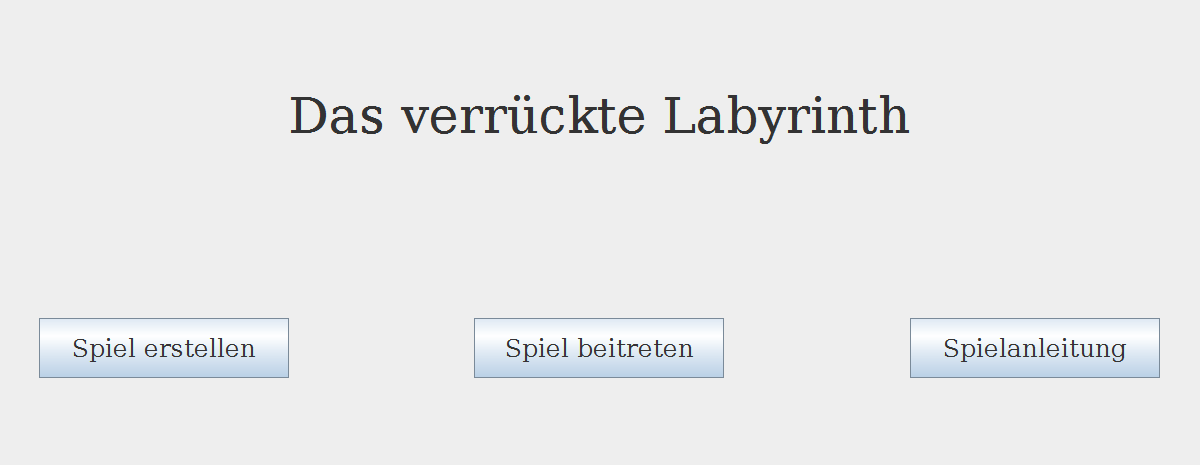
\includegraphics[scale=0.25]{Bilder/bild1.png}
				\end{block}		
			\end{frame}
			%========================================================
			%+++++++++++++++++++++++++++++++++++++++++++++++++++++++
			%FRAME 2:
		    \label{Frame2}	
			\begin{frame}
				\frametitle{create New Game}
				\begin{block}{New Game}
					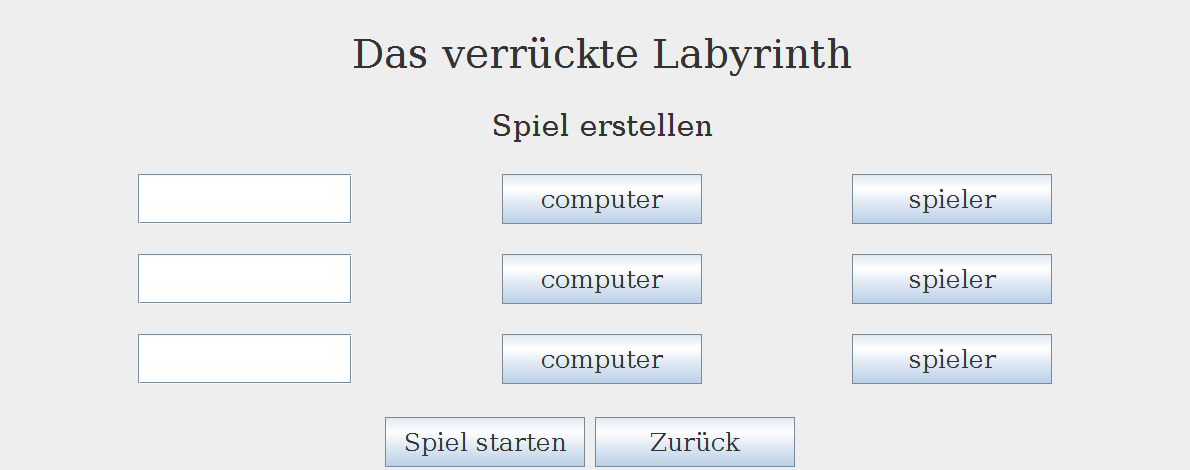
\includegraphics[scale=0.25]{Bilder/bild2.png}
				\end{block}		
			\end{frame}
			%========================================================			
			%+++++++++++++++++++++++++++++++++++++++++++++++++++++++
			%FRAME 3:
		    \label{Frame3}	
			\begin{frame}
				\frametitle{Field}
				\begin{block}{Field}
					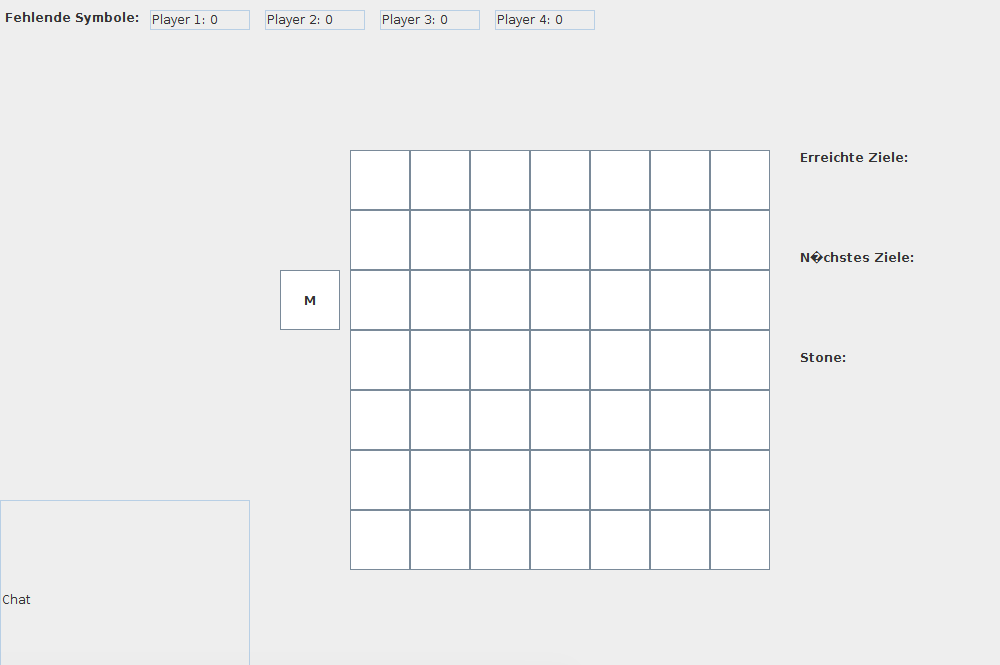
\includegraphics[scale=0.27]{Bilder/bild3.png}
				\end{block}		
			\end{frame}
			%========================================================	
\end{document}	